%%%%%%%%%%%%%%%%%%%% author.tex %%%%%%%%%%%%%%%%%%%%%%%%%%%%%%%%%%%
%
% sample root file for your "contribution" to a contributed volume
%
% Use this file as a template for your own input.
%
%%%%%%%%%%%%%%%% Springer %%%%%%%%%%%%%%%%%%%%%%%%%%%%%%%%%%%%%%%%%


\title{Structural Systems}
\author{
    \textbf{Gregory G. Deierlein} 
    \and Ertugrul Taciroglu}
\tocauthor{}
\authorrunning{Deierlein and Taciroglu}
%\institute{Name of First Author \at Name, Address of Institute, %\email{name@email.address}
%\and Name of Second Author \at Name, Address of Institute %\email{name@email.address}}
%
% Use the package "url.sty" to avoid
% problems with special characters
% used in your e-mail or web address
%
\maketitle

Response simulation of structural systems is an essential component of natural hazards engineering to quantify the effects of gravity loads, earthquake ground motions, wind and water flows, and other loads on buildings, bridges, piers, pipelines and other constructed facilities. Founded on the principles of structural mechanics, structural response simulation methods encompass a broad range of computational approaches, ranging from simplified phenomenological models to detailed continuum finite-element methods. The required simulations encompass a broad range of structural materials, systems, and scales. Construction materials include wood, masonry, concrete, steel, and other materials configured in multiple ways. The scale of simulations ranges from detailed finite-element models of structural components and connections up through complex 3D structural systems and, in the case of regional simulations, large inventories or networks of structures.

The field of structural and finite-element analysis is well established and documented in academic research papers and textbooks, and it is complimented by a multitude of research and commercial software of varied capabilities. This review is limited in scope to the subset of structural simulation methods and software technologies that are most directly relevant to natural hazards engineering, particularly those that are well suited to the research objectives and questions in the NHERI Science Plan. 

\section{Input and Output Data}
\label{sec:resp_struct_io}

In the context of natural hazards engineering, structural response simulations entail the development and analysis of idealized structural models to assess the structural responses necessary to evaluate damage and resulting consequences (life-safety risks, economic loss, downtime, etc.) to constructed facilities and systems. In developing structural response models, it is important to clearly define the objectives and scope of the model, specifically with regard to how the hazard loading effects will be incorporated and how the results of the analyses will be used. At one extreme, structural response analyses may involve high-resolution models to interrogate local (pointwise) response of structural materials and components. At the other extreme, highly idealized models of building systems may be used to evaluate economic losses and downtimes for regional assessments of large building inventories. Obviously, the goals of the simulation will dictate the type and resolution of the model employed, including how the input hazard is characterized and how the simulation output will inform downstream calculations.

In earthquake engineering applications, the loading input for structural simulations is usually earthquake ground shaking, which is described in terms of one or more IMs (e.g., spectral acceleration, spectral displacement, duration, etc.) or ground-motion seismograms. In some cases, the earthquake input may be characterized by input ground deformations, such as for buried pipelines and tunnels or structural foundations. In wind engineering, the loading input is typically equivalent static wind pressures or response histories of wind pressures, the latter being more important for flexible structures that interact dynamically with the wind. For assessment of storm surge and tsunami inundation, the loading input is usually equivalent static water pressures or debris flow forces. 

Traditionally, structural response simulation has focused on structural framing components and systems; more holistic risk assessments require modeling of so-called nonstructural components that can affect the structural response and final damage state. For wind and water inundation flows, the interaction between the wind/water flows and the architectural cladding, partition walls, and other surfaces is particularly important. For earthquake engineering, architectural cladding and partition walls are important to model for certain types of light-frame construction because these components can provide significant strength and stiffness (e.g., wood-frame residential houses).

\section{Modeling Approaches}
\label{sec:resp_struct_methods}

As illustrated in Figure \ref{fig:response_ModelTypes}, models for nonlinear analysis of structures can range from uniaxial spring or hinge models, to more fundamental fiber section and continuum finite-element models. In general, all models are phenomenological in that they rely on empirical calibration to observed behavior at some level of idealization. The concentrated models (see Figure \ref{fig:response_ModelTypes}a-b) are highly phenomenological in that the underlying functions that describe the structural behavior are based on semi-empirical calibration to overall component behavior \cite[e.g.][]{ibarra2005hysteretic, folz2001saws, lowes2003modeling, do2018damage}. While Figure \ref{fig:response_ModelTypes} illustrates these as moment-rotation hinge models, the concentrated springs can apply to any univariate response quantity, e.g., axial or shear springs. At the other extreme, the continuum finite-element models (see Figure \ref{fig:response_ModelTypes}e) are calibrated at the material level \cite[e.g.][]{lemaitre1990mechanics, dettmer2004theoretical, lee1998plasticdamage, maekawa2003nonlinear}, where the kinematics and equilibrium of the components are represented more directly by the model formulation. As such, the continuum models are more adaptable to different geometries and loading regimes; however, to the extent possible, the models should be validated against test data that represents the governing phenomena in the structural components being modeled. In between the concentrated hinge and continuum models are fiber section or fiber hinge models (see Figure \ref{fig:response_ModelTypes}c-d), where kinematic assumptions (such as plane sections remain plane) are used to relate uniaxial material response to generalized strains and stress resultants (e.g., moment-curvature) at member cross sections. The uniaxial material models that comprise fiber models can be calibrated based on the uniaxial material stress-strain behavior \citep[e.g.,][]{mander1988theoretical, dodd1995model, menegotto1973method} or alternatively on quasi stress-strain, where the properties are adjusted to account for phenomena such as steel reinforcing bar buckling \citep[e.g.,][]{kunnath2009nonlinear,dhakal2002pathdependent}.

\begin{figure}[htb]
    \centering
    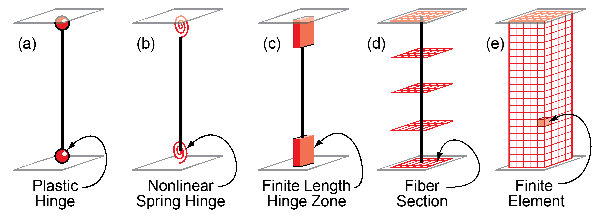
\includegraphics[width=1.0\textwidth, angle = 0]{Figures/ModelTypes.pdf}
    \caption{Range of structural model types \citep{deierlein2010nonlinear}}
    \label{fig:response_ModelTypes}
\end{figure}

The choice of model type for a given application involves a balance between reliability, practicality, and computational efficiency, subject to the capabilities of available software and computational resources. The optimal model type depends on many factors, including the structural system and materials, governing modes of behavior, the expected amount of nonlinearity, and the level of detail available for the input and output data. The reliability of the model comes from its ability to capture the critical types of deformation that are of interest to the modeler and control the response. 

In recent years, applications to performance-based earthquake engineering have led to major advancements in the development and calibration of nonlinear structural analysis models to simulate the response of buildings, bridges, and other structures from the onset of damage up through collapse. A series of recent NEHRP publications review structural models and modeling parameters for nonlinear analysis to support seismic evaluation, retrofit, and design of buildings \citep{nist2017guidelines,nist2017guidelinesa,nist2017guidelinesb}. These NIST documents summarize models and parameters, along with references to many of the underlying research publications, for concrete and steel moment frames, steel concentrically braced frames, concrete shear walls, reinforced masonry walls, and light-frame wood shear walls. A NIST technical brief \citep{deierlein2010nonlinear} provides a broader review of nonlinear analysis methods with a summary of proposed research and development needs for performance-based seismic engineering of buildings. Other resources on nonlinear modeling and analysis include: PEER/ATC report on tall buildings \citep{malley2010modeling}, \cite{spacone2004nonlinear} on composite steel-concrete structures, and \cite{nurbaiah2017modelling} on masonry infilled RC frames.

A detailed performance-based modeling and analysis guidelines for bridges is described in a PEER report by \cite{aviram2008guidelines}, which targets reinforced concrete (single- or multi-span) bridges common in California \citep{nbi2016national}. An example of the components involved in modeling of a typical bridge is shown in Figure \ref{fig:response_BridgeModel}. Research cited in the Aviram report and publications since then address structural modeling details for bridges related to: (1) straight and skew angled abutment backfill models \citep{shamsabadi2010validated}: (2) abutment kinematic interaction models \citep{zhang2002kinematic}: (3) shear key models \citep[e.g.][]{silva2009seismic}; (4) pile-soil interaction models for conventional \citep{hutchinson2001inelastic, taciroglu2006robust}, group \citep{lemnitzer2010nonlinear} and large-diameter \citep{khalili-tehrani2014nonlinear} piles; (5) in-span hinge models \citep{hube2008experimental}; and (6) column models \citep{terzic2015concrete, xu2011hysteretic}. The aforementioned models have been used in studies that furthered the state-of-the-art, which include work by \cite{kaviani2014performancebased}, who targeted skew bridges, \cite{omrani2015guidelines}, who comprehensively examined and improved upon the bridge PBSA guidelines by \cite{aviram2008guidelines}, and \cite{omrani2017variability}, who examined fragility sensitivities to abutment modeling uncertainties. In all these studies, the analysis tool of choice has been OpenSees \citep{mckenna2011opensees} wherein most, if not all, of the aforementioned models are publicly available. 

\begin{figure}[htb]
    \centering
    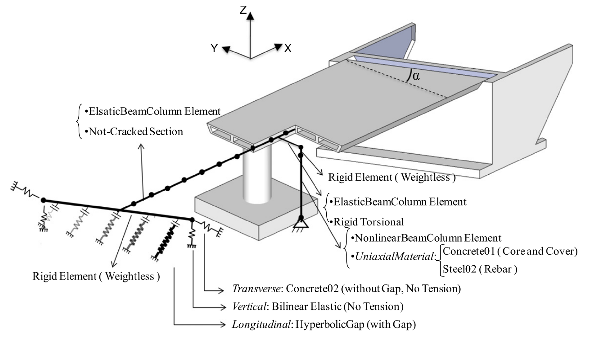
\includegraphics[width=1.0\textwidth, angle = 0]{Figures/BridgeModel.pdf}
    \caption{Schematic view of a generic bridge numerical model in OpenSees \citep{kaviani2012seismic}}
    \label{fig:response_BridgeModel}
\end{figure}

Most natural hazards research on nonlinear response simulation of structures is related to earthquake engineering where addressing inelastic response has long been recognized as a necessity under design ground motions. In contrast, inelastic structural effects tend to be less pronounced for evaluation of gravity, wind, and other loading effects. In the case of storm-driven wind and wave loading or tsunami inundation, the largest nonlinear behavior involves the loading due to the dynamic fluid (air or water) flows and their interaction with the structure. Examples of recent research to study the response of structures to fluid flows include \cite{minjie2014modeling, minjie2018validation, ataei2015fragility, petrone2017fragility, madurapperuma2013response, attary2016methodology}.

Repeated nonlinear response history analyses for constructing seismic fragilities or for performing simulations of regionally distributed systems typically require large-scale computational resources. Due to the granular nature of each structural analysis, the required computations are embarrassingly parallel (i.e., perfectly scalable in a parallel computing sense). Apart from the computational requirements, analyses of buildings, bridges, or other distributed infrastructure requires consideration of correlations in the hazard demands (e.g., earthquake ground motions) across the region along with correlations of the structural system response. Such regional-scale analyses are uncommon and not standard, but various attempts have been made \citep[see e.g.][]{miller2015estimating}.

\section{Software and Sytems}
\label{sec:resp_struct_tools}

While there are a large number of available software systems with various capabilities, this summary focuses on software programs that are well-suited and widely used in research related to natural hazards engineering. Emphasis is on open-source software currently available and supported on the NHERI DesignSafe computing platform along with a few widely used commercial codes.
% \newline

\paragraph{OpenSees} The Open System for Earthquake Engineering Simulation (\citeprgm{OpenSees}) is an open-source object-oriented software framework for simulating the seismic response of structural and geotechnical systems. OpenSees was developed and is maintained by the Pacific Earthquake Engineering Research (PEER) Center for research in performance-based earthquake engineering and is widely used and contributed to by researchers from around the world. OpenSees has advanced capabilities for modeling and analyzing the nonlinear response of structural systems using a wide range of material models, beam-column elements and continuum elements, and solution algorithms. The software is designed for parallel computing to allow scalable simulations on high-end computers or for parameter studies. The software is available on DesignSafe and can be downloaded to run on Linux, Windows, or Mac OS (\url{http://opensees.berkeley.edu/})

\paragraph{LS-DYNA} \citeprgm{LS-DYNA} is a general-purpose finite element program capable of simulating complex real-world problems with primary users from the automobile, aerospace, construction, military, manufacturing, and bioengineering industries. It has nonlinear frame and continuum finite elements, with material models for steel, concrete, and soils along with fluids. LS-DYNA's origins lie in highly nonlinear, transient dynamic finite-element analysis using explicit time integration, and it is optimized for shared and distributed memory Unix, Linux, and Windows-based platforms. The software is maintained and marketed by Livermore Software Technology Corporation, with licensing available to both the commercial and academic markets. It is available on DesignSafe for users with an academic license. (\url{http://www.lstc.com/products/ls-dyna}) 
% \newline

\paragraph{FEAP} The Finite Element Analysis Program (\citeprgm{FEAP}) is a general-purpose finite-element program for solving nonlinear, static, and transient partial differential equations. Its primary applications are directed to the solution of problems in solid mechanics; however, the system may be extended to solve problems in other subject areas by adding user developed modules to address problems in fluid dynamics, flow through porous media, thermo-electric fields, and others. The software is available to run on UNIX/Linux/Mac or Windows environments (see \url{http://feap.berkeley.edu/})
% \newline

\paragraph{Other Commercial Software} The following is a list of other commercial software, with simulation capabilities for natural hazards engineering commonly used in both industrial and academic research.

\begin{itemize}
    \item SAP 2000, ETABS, PERFORM3D (\url{https://www.csiamerica.com} )
    \item ABAQUS Unified FEA (see \url{https://www.3ds.com/products-services/simulia/products/abaqus/}).
    \item LARSA (\url{https://www.larsa4d.com/})
    \item Marc (\url{http://www.mscsoftware.com/product/marc})
    \item DIANA (\url{https://dianafea.com})
\end{itemize}

\section{Research Gaps and Needs}
\label{sec:resp_struct_gaps}

While computational tools for simulation of structural materials and systems are fairly mature, there are still significant limitations in the modeling capabilities along with the continuing need for improved calibration and validation of existing models. The limitations and needs depend on the scale and resolution of the models, i.e., whether one is interested in detailed models of structural material and components to examine localized behavior or less detailed models that can reliably simulate the behavior of complete structural systems (buildings, bridges, etc.) or large inventories of systems (e.g., building inventories or geographically distributed infrastructure systems). 

At the detailed level, there are continuing needs to develop, implement, and validate continuum finite-element models that can simulate nonlinear behavior and damage to structural materials and components under random cyclic loading, including interfaces and interaction between materials. Models for steel and other ductile materials are fairly well established for simulating large plastic strains and deformations (e.g., to simulate local and overall buckling [see \cite{n.i.s.t.-a.t.c.2018blind}], whereas methods to reliably capture fracture under cyclic inelastic loading are still evolving. For other structural materials, including reinforced concrete, wood-based materials, and masonry, many challenges remain to reliably simulate inelastic damage and degradation as seen in physical tests. In addition to the models themselves, further research and development are needed to implement and validate models in open-source software to run on high-performance computing resources to broaden their impact in natural hazards engineering.

At the large-scale system or distributed inventory/system level, there is a need for systematic approaches that develop, calibrate, and manage models computationally efficient enough to be deployed at scale, which also capture accurately the dominant behavioral effects. For such applications, many of the challenges are more related to supporting modeling and data management tools as much as the models themselves. A related need is to develop inventory data with reliable descriptions of the systems that includes information on the uncertainties and correlations in those uncertainties.

